%!TEX root = ../../report.tex

\subsection{Graphic Tools} % (fold)
\label{sub:graphic_tools}
There are several Application Programming Interfaces (APIs) for graphic content creation, but the most known ones are DirectX and OpenGL. 

DirectX is a collection of multimedia APIs created by Microsoft for their platforms. It includes the Direct3D API. This tool has evolved very much since it was released and supports the state of techniques such as hardware acceleration and so forth.  On the other hand this system is only supported by Microsoft platforms and since this work should not be limited to the Microsoft platforms, this tools will not be used. 

OpenGL is an open-source library that is widely used. This system will be better explained in the next section.

\subsection{Modern OpenGL} % (fold)
\label{sub:modern_opengl}


OpenGL is a well known cross-platform API created by Silicon Graphics Computer Systems with Version 1.0 released in July of 1994 for 3-D Graphics and Imaging. It is a streamlined and hardware-independent interface that can be implemented on many different types of graphics hardware. It is also independent of the machine's operative and windowing systems.

Major changes has been imposed to this library from its early versions and this section covers the modern version of OpenGL after version 3.2.

OpenGL provides a small set of geometric primitives - points, lines, triangles and patches that are specified by their vertices. From this set of geometric primitives all geometry is constructed, both in 2D and 3D. 

There are some steps that are performed to render an image, and OpenGL follows the pipeline in Figure~\ref{fig:OGLPipeline}. While some of steps are fix and are automatically executed, other steps are programmable, which allows the developers to program directly to the GPU. This code that runs on the GPU is called shader. Shaders can be thought of as small programs that are specifically compiled for the GPUs\cite{shreiner2013opengl}.

First the model is created from geometric primitives and it is the input for the pipeline (\emph{Vertex Data} on Figure~\ref{fig:OGLPipeline}). 

\begin{figure}[htbp]
	\centering
	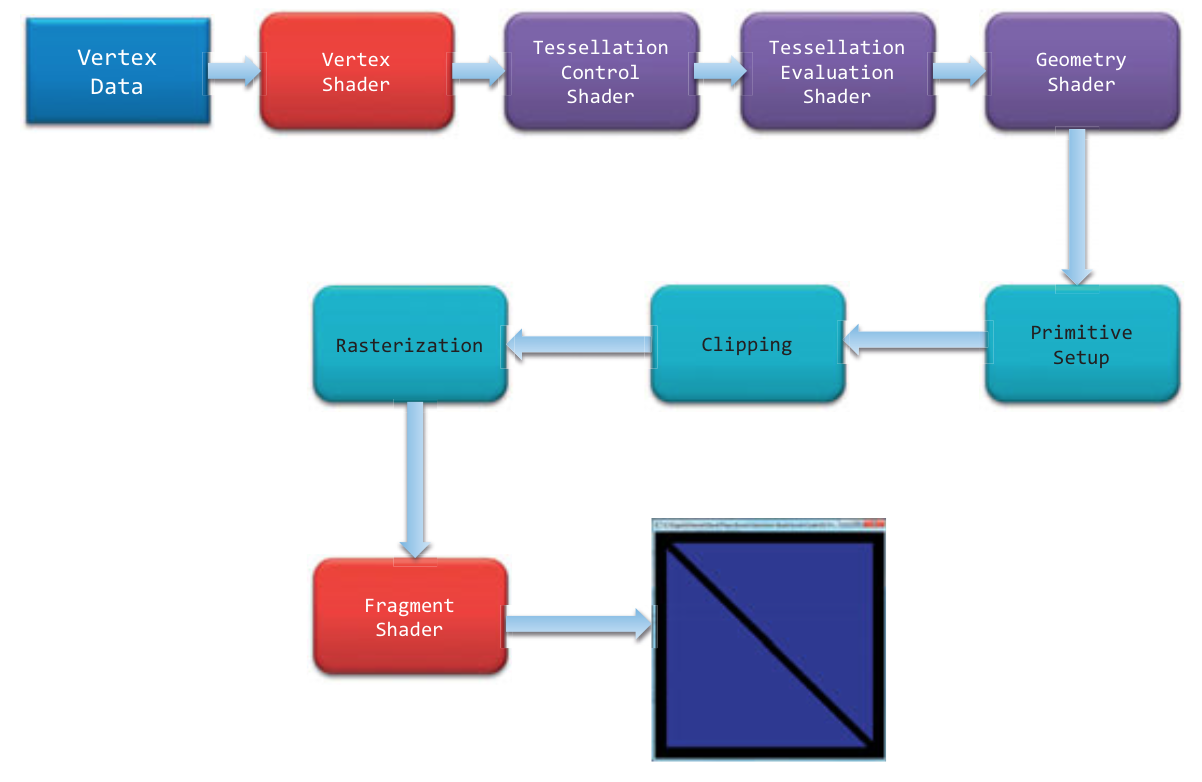
\includegraphics[width=0.95\textwidth]{img/OpenGL/pipeline.png}
	\caption{OpenGL Pipeline \cite{shreiner2013opengl}}
	\label{fig:OGLPipeline}
\end{figure}


The first step of the pipeline is the Vertex Shader that process the data associated with each vertex. 

After, there are three optional shaders. In this three there are two Tessellation Shaders. With this shaders simple geometries can be tessellated and increase of the number of primitives to improve the models dynamically.

The third optional shader is the Geometric Shader that allows the additional processing of geometric primitives and also including the creation of new primitives.

Until now all steps work with vertices. After those steps there are three fixed steps, primitive assembly, clipping and rasterization that assembly the vertices into primitives, clip the geometry cutting the parts that falls off the ``screen'' and the generation of fragments, respectively.

A fragments is a ``‘\emph{candidate pixel}’, in that pixels have a home in the framebuffer, while a fragment still can be rejected and never update its associated pixel location'' \cite{shreiner2013opengl}.

\subsubsection{Vertex Shaders} % (fold)
\label{sub:vertex_shaders}
can be very simple, from a \emph{pass-through shader} that just copies the data to the next step to very complex ones.

These shaders are used to perform computations to calculate the position of the vertices in screen coordinates, assign vertex's color using lightning computations, etc..

Vertex Shaders have some limitations, they cannot create additional geometry and cannot access data of other vertices. They can just process the data of the current vertex and the number of vertices after this step is the same as before.

% subsection vertex_shaders (end)

\subsubsection{Tessellation Shaders} % (fold)
\label{sub:tesselation_shaders}
are very different form the previous ones. This shaders address some of limitations presented before.
This shaders work with a geometric primitive called a \emph{patch}. A patch is a list of vertices that preserves their order during processing. Each patch can have an arbitrary number of vertices that have to be specified before drawing, in contrast to the other primitives that have a specific number of vertices.

\subsubsection{Tessellation Control Shader} % (fold)
\label{ssub:tesselation_control_shader}
	 defines the layout of the output through the generation of the tessellation output-patch vertices and the specification of the tessellation level factors. The output-patch vertices is the list of vertices that results after the input vertices have been processed. The tessellation level factor defines how much the output patch is tessellated. 

	OpenGL supports three tessellation domains: a quadrilateral, a triangle, and a collection of isolines \cite{shreiner2013opengl}. To control the amount of tessellation two sets of values are assigned, the outer-tessellation values and the inner-tessellation values. This values define how the perimeter or the interior of the domain are subdivided respectively. 

	As an example, Figure~\ref{fig:ex1TessControl} shows a triangular domain with the following tessellation levels. 
	\begin{lstlisting}[frame=single,language=C++]
	gl_TessLevelOuter[0] = 6;
	gl_TessLevelOuter[1] = 5;
	gl_TessLevelOuter[2] = 8;

	gl_TessLevelInner[0] = 5;
	\end{lstlisting}

In this example three outer control values are used, each one correspond with one side of the triangle and one inner value. Each outer value defines the number of divisions that its correspondent side has. 

\begin{figure}[htbp]
	\centering
	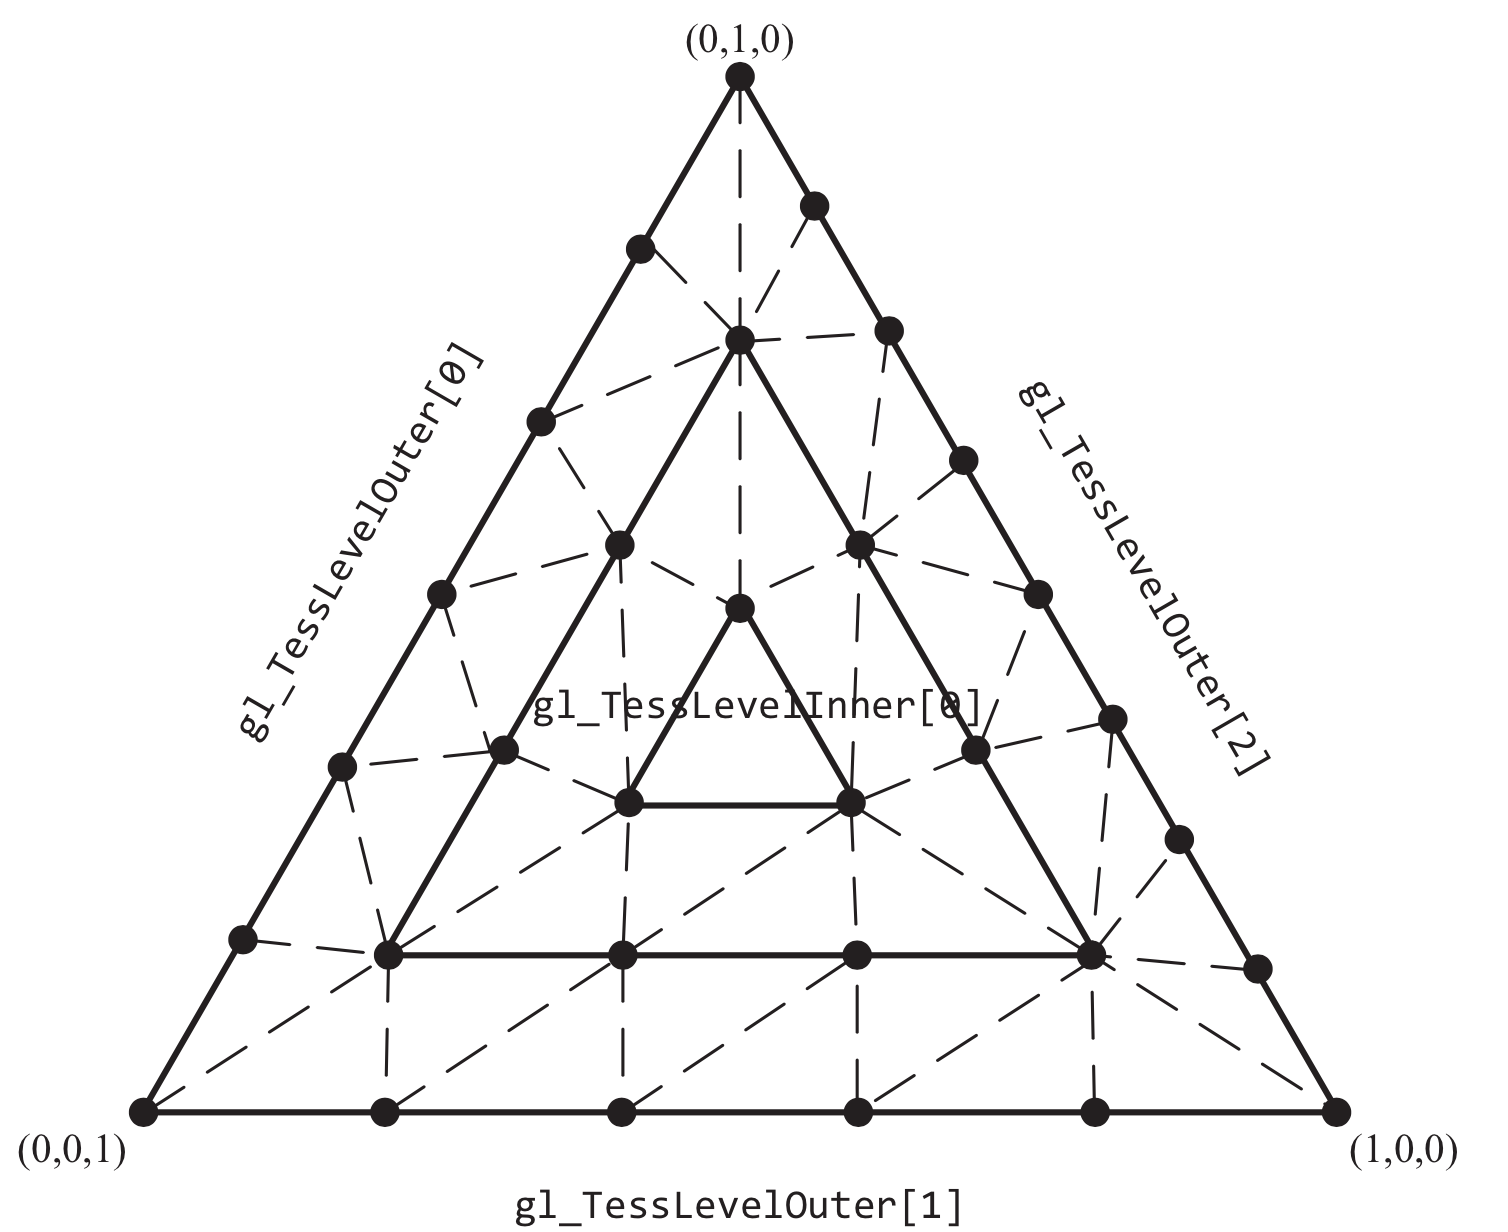
\includegraphics[width=0.65\textwidth]{img/OpenGL/TessShaderEx1.png}
	\caption{Example for tesselation control with triangular domain \cite{shreiner2013opengl}}
	\label{fig:ex1TessControl}
\end{figure}


%\begin{wrapfigure}{r}{0.5\textwidth}
%	\vspace{-15pt}
%    \centering
%	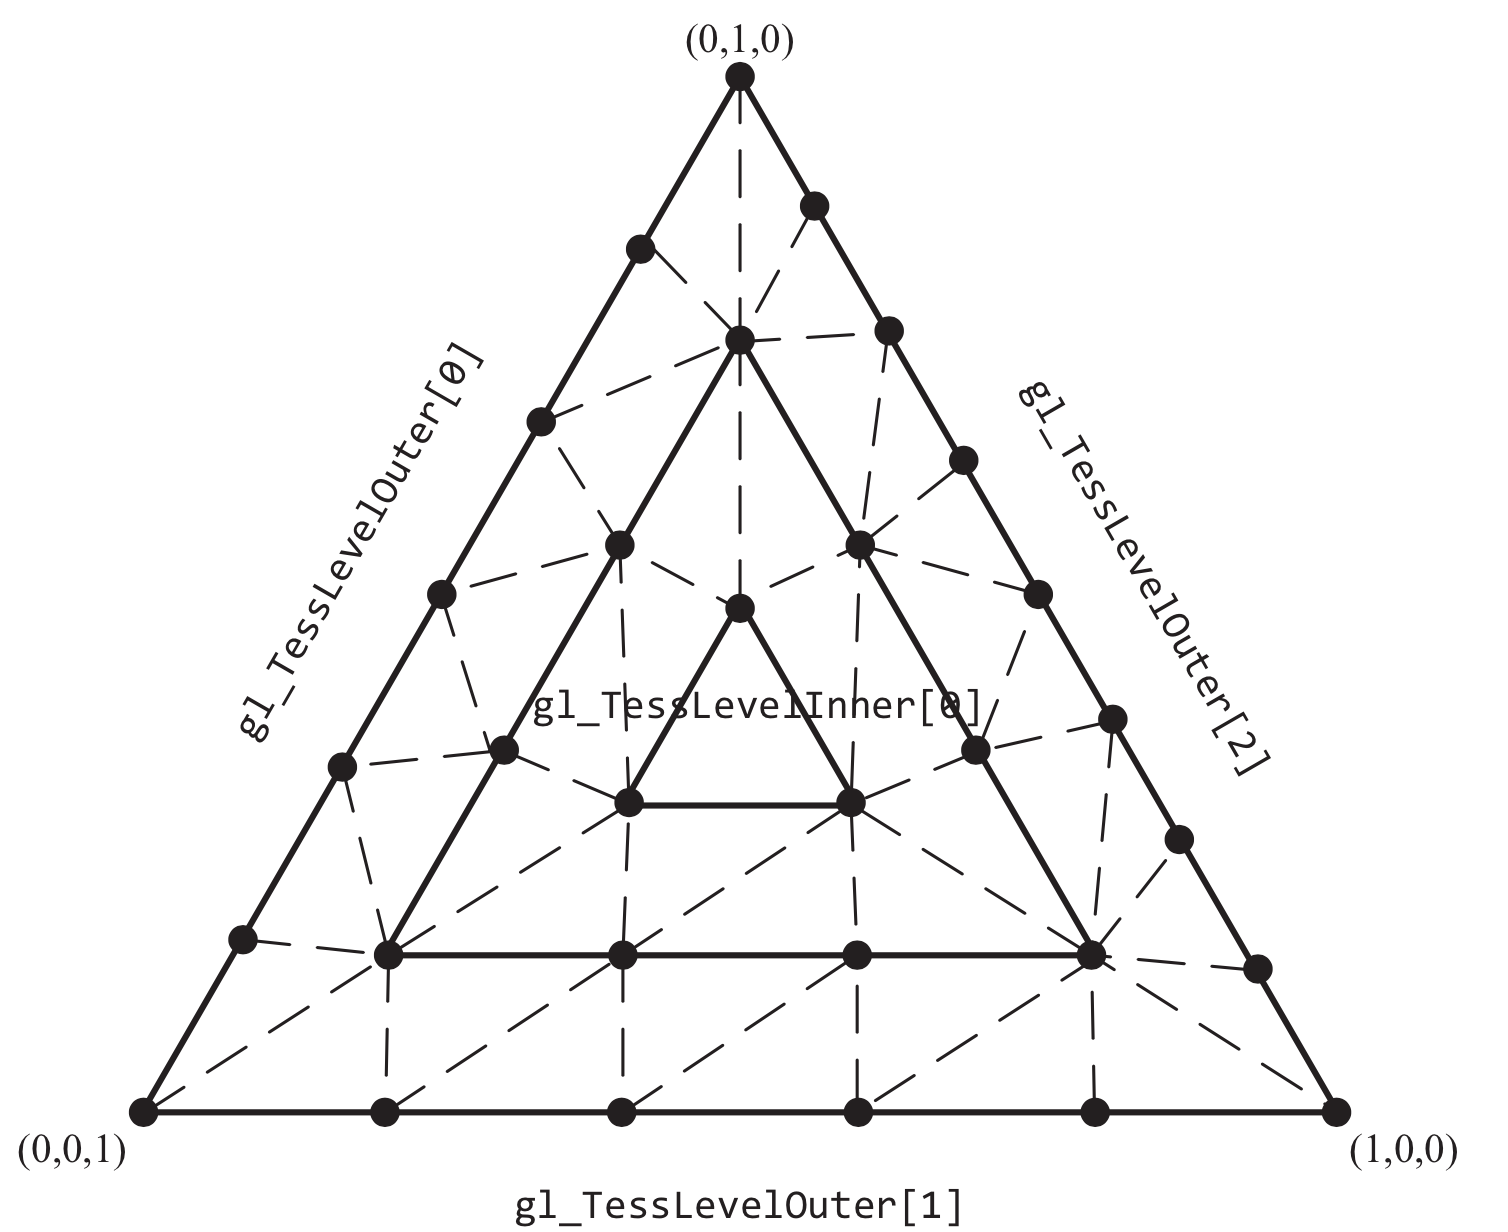
\includegraphics[width=0.5\textwidth]{img/OpenGL/TessShaderEx1.png}
%	\caption{High Level Architecture}
%	\label{fig:architecture}
%	\vspace{-15pt}
%\end{wrapfigure}

% subsubsection tesselation_control_shader (end)

\subsubsection{Tessellation Evaluation Shaders} % (fold)
\label{ssub:tesselation_evaluation_shaders}
Tessellation shaders work with the output of the previous phase. Here the vertex positions are computed from the tessellation computed before. It is is basically responsible for the computation of the vertices' screen positions from the layout defined.

% subsubsection tesselation_evaluation_shaders (end)

% subsection tesselation_shaders (end)

\subsubsection{Geometry Shaders} % (fold)
\label{sub:geometriy_shaders}

Geometry Shaders are the first shaders that access the complete primitive as a list of vertices and with that it is allowed to do different actions that require this access to information. The amount of output can be variable so both \emph{culling geometry} and \emph{geometry amplification}, respectively output less vertices that the input and output more vertices than the input. Also in this shaders the primitives type can be modified, i. e. the input can be \emph{quads} and the output be a \emph{triangle\_strip}.

Geometry shaders however have a limitation. Each call of a geometry shader have a maximum number of vertices that it can output. This limitation could be important for the implementation of geometry amplification. This maximum number is hardware dependent and varies with the size of the output buffer that is used by the GPU to support geometry shaders. OpenGL specification since version 4.3 imposes 256 as the minimum number of vertices supported.

% subsection geometriy_shaders (end)

\subsubsection{Fragment Shaders} % (fold)
\label{sub:fragment_shaders}
This shaders implement the last phase of the pipeline. Here the fragment's final color is computed and also the depth value.

Fragment Shaders are useful to implement texture mapping or lights, for instance.

% subsection fragment_shaders (end)
% subsection modern_opengl (end)